\documentclass{article}
\usepackage[utf8]{inputenc}
\usepackage[spanish]{babel}
\usepackage{listings}
\usepackage{graphicx}
\graphicspath{ {images/} }
\usepackage{cite}
\usepackage{subcaption}

\begin{document}

\begin{titlepage}
    \begin{center}
        \vspace*{1cm}
            
        \Huge
        \textbf{Proyecto final}
            
        \vspace{0.5cm}
        \LARGE
        Laberintos 
            
        \vspace{1.5cm}
            
        \textbf{Emmanuel Garay Rivera\\
        Sofía Marín Cacante}
            
        \vfill
            
        \vspace{0.8cm}
            
        \Large
        Despartamento de Ingeniería Electrónica y Telecomunicaciones\\
        Universidad de Antioquia\\
        Medellín\\
        Marzo de 2021
            
    \end{center}
\end{titlepage}

\tableofcontents
\newpage
\section{introduccion}\label{intro}
Un juego de laberintos cambiantes que en cada reto superado, aumente su dificultad. 

\section{Explicación} \label{contenido}
Con imágenes y algunos ejemplos se quiere mostrar el objetivo y la implementación del juego.
\subsection{Objetivo e implementación.}
Para los laberintos se definirá una meta, la posición inicial del jugador o personajes, el tamaño del tablero que representará el laberinto en la matriz Mnxn (siendo n el número de filas y columnas) y un conjunto de rutas posibles; la ruta que resuelve el laberinto (ruta entre la meta y el personaje) no debe superar ((Mnxn)/n-1) y debe ser la única ruta que llegue al borde del laberinto. Lo anterior se ejemplificará en la figura (\ref{fig:figura2}).

\begin{figure}[h]
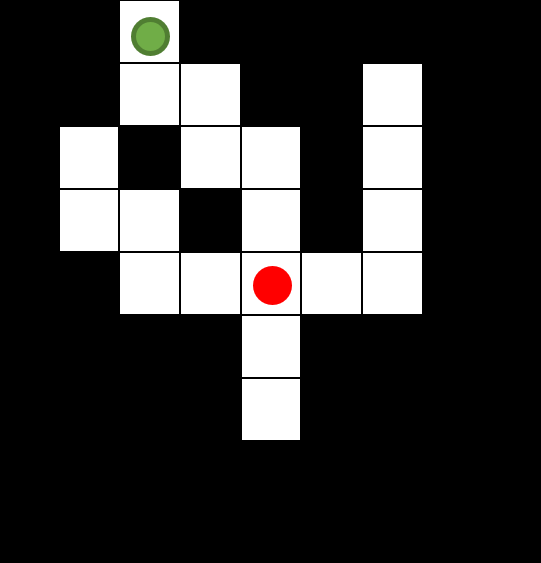
\includegraphics[width=4cm]{figura2.png}
\centering
\caption{Ejemplo de un camino}
\label{fig:figura2}
\end{figure}


Otro punto importante es que cada t de tiempo se crea otro escenario teniendo en cuenta la posición actual del personaje, esto sucede en un mismo nivel, ya que cuando el personaje llega a la meta y pasa de nivel, el tamaño del escenario será el cuádruple del anterior. 

Además, se busca que n sea múltiplo de 3 para que el programa en cada nivel, inicialice al juagador o personaje en el centro.

\newpage

\subsection{Ejemplos}
El primer escenario será de 9x9, cada t de tiempo las rutas van a cambiar hasta que el personaje llegue a la meta, cuando esto pase el personaje llegará a un nuevo nivel y un nuevo escenario de 18x18 en el que tendrá el mismo objetivo pero con la dificultad de un escenario más grande.

\begin{figure}[h!]
    \centering
    \begin{subfigure}[b]{0.45\linewidth}
        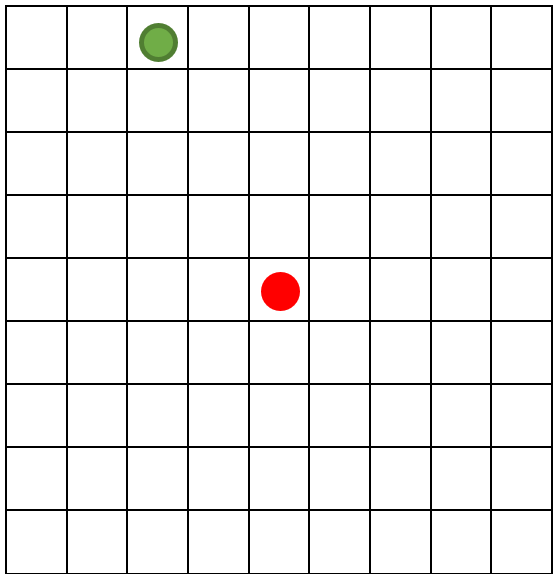
\includegraphics[width=\linewidth]{figura1.png}
        \caption{Ejemplo nivel 1}
        \label{fig:figura1}
    \end{subfigure}

    \begin{subfigure}[b]{0.45\linewidth}
        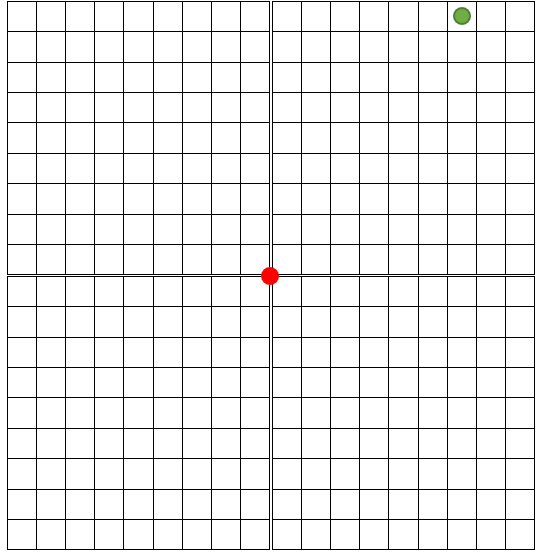
\includegraphics[width=\linewidth]{figura3.png}
        \caption{Ejemplo nivel 2}
        \label{fig:figura3}
    \end{subfigure}
\end{figure}


\end{document}
